\subsection{CPU}

These charts represent the \gls{cpu} usage of clients and servers during ephemeral and persistent experiments.

They follow a similar pattern to the latency and throughput results, \gls{http}/1 has the lowest \gls{cpu} usage, while \gls{http}/3 has the highest.

\gls{http}/3 is the worst since it has to deal with QUIC’s cryptography, sending and receiving of \gls{udp} packets, and maintaining internal QUIC state. \gls{http}/2+\gls{tls} and \gls{http}/1+\gls{tls} is better than \gls{http}/3, since they perform better in a reliable network, as stated before. Finally, \gls{http}/1 and \gls{http}/2 are the most performing since they do not have to deal with data encryption and \gls{tls}  handshake overhead.

Server \gls{cpu} usage is mirrored with client’s. This can be explained by the fact that the server response has the same size as the client request, resulting in the same usage of \gls{cpu} since they have to perform the same operations to be able to send data.

\clearpage

\begin{figure}[h!]
    \centering
    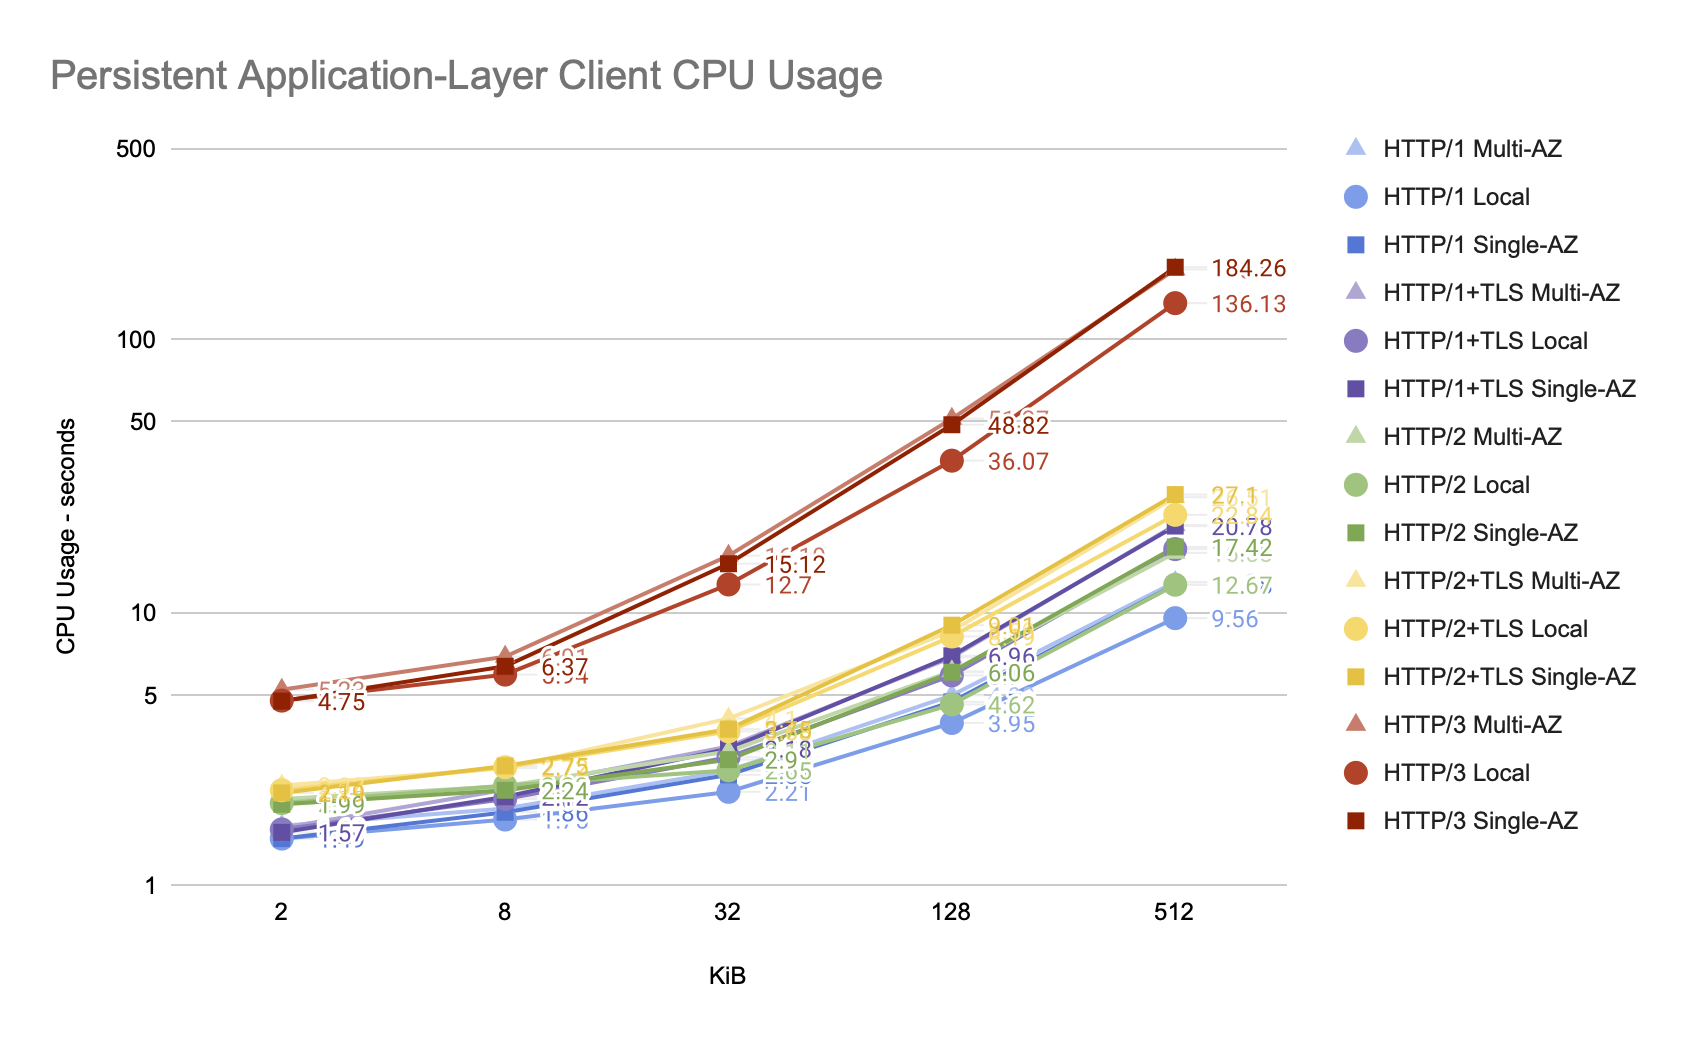
\includegraphics[width=\linewidth]{figures/charts/Persistent Application-Layer Client CPU Usage.png}
    \caption{Persistent Application-Layer Client CPU Usage}
    \label{fig:persistent_client_application_cpu}
\end{figure}

\begin{figure}[h!]
    \centering
    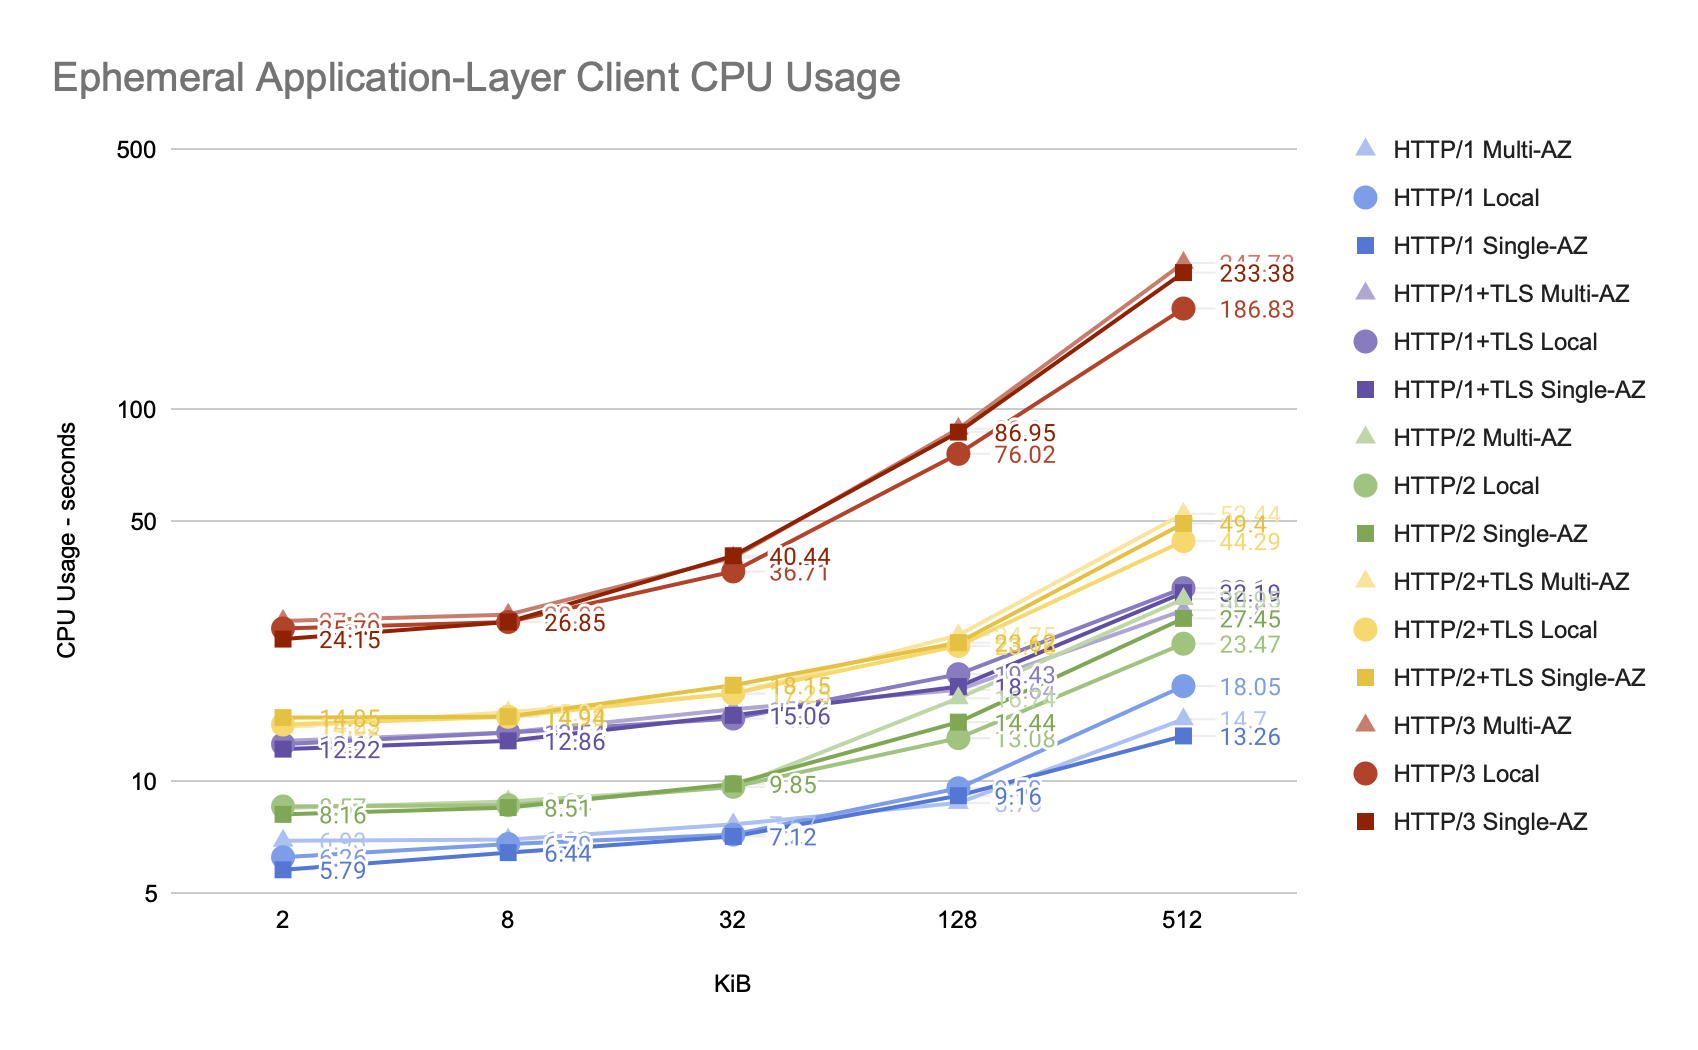
\includegraphics[width=\linewidth]{figures/charts/Ephemeral Application-Layer Client CPU Usage.png}
    \caption{Ephemeral Application-Layer Client CPU Usage}
    \label{fig:ephemeral_client_application_cpu}
\end{figure}

% \begin{figure}[h!]
%     \centering
%     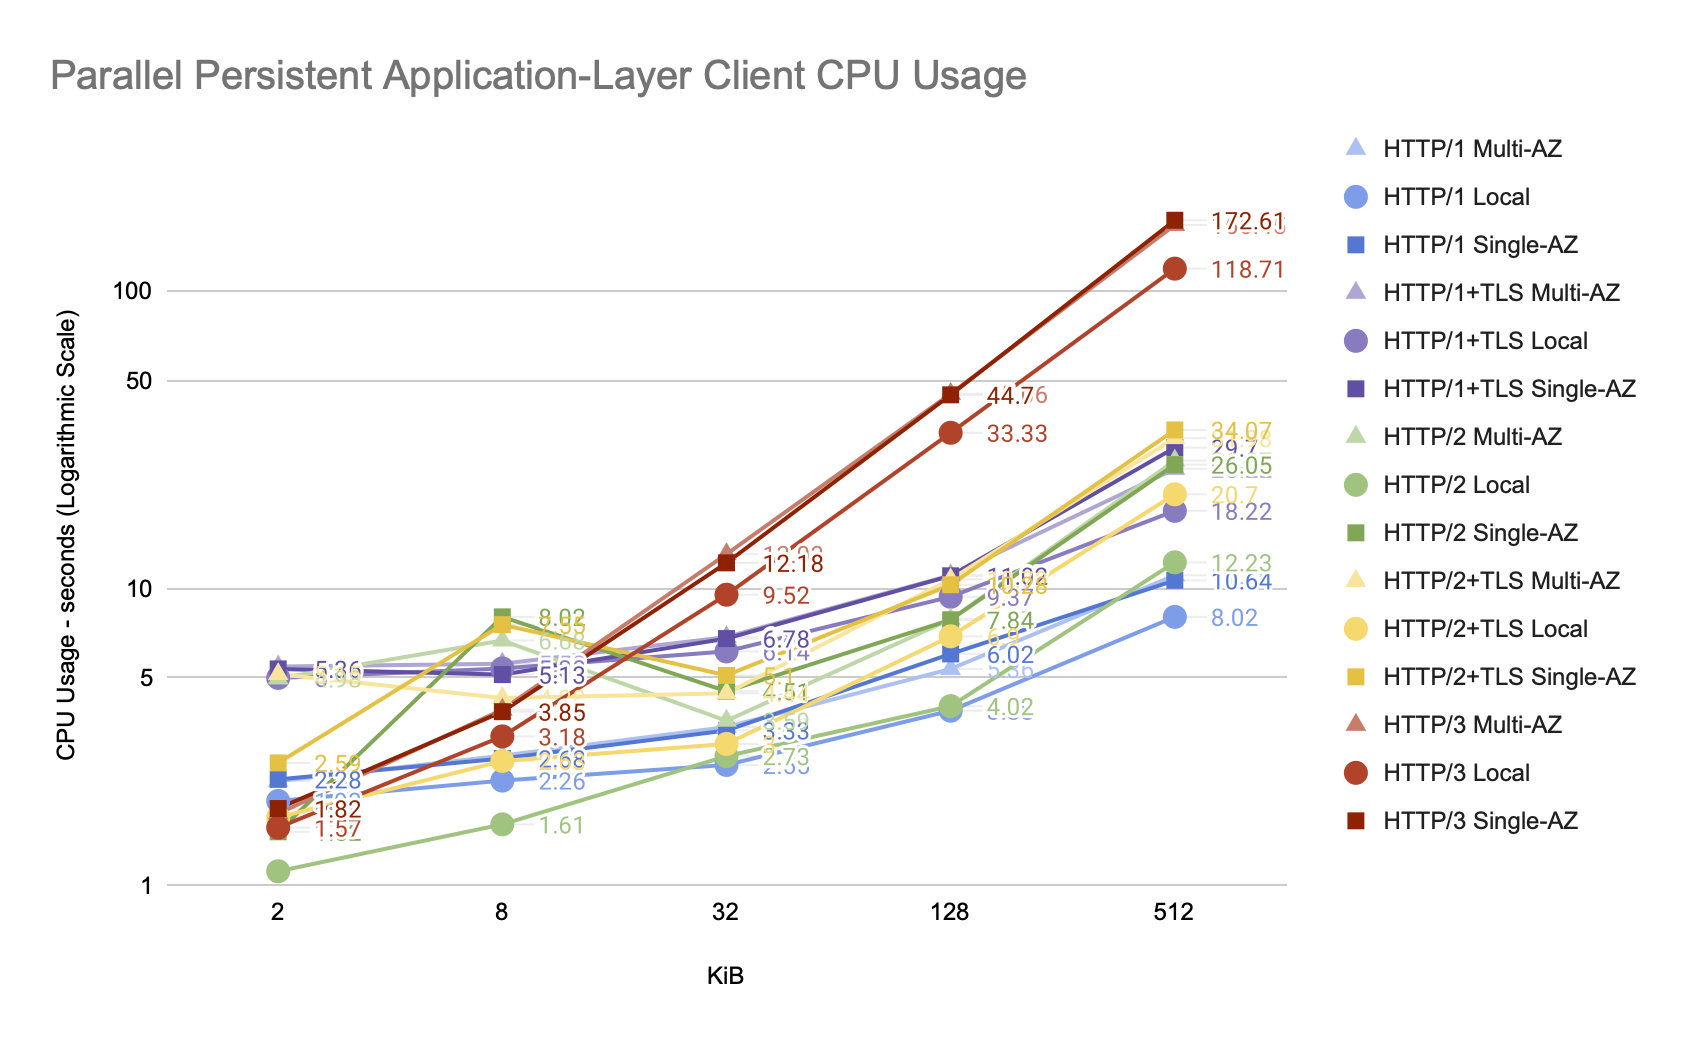
\includegraphics[width=\linewidth]{figures/charts/Parallel Persistent Application-Layer Client CPU Usage.png}
%     \caption{Parallel Persistent Application-Layer Client CPU Usage}
%     \label{fig:parallel_client_application_cpu}
% \end{figure}

\begin{figure}[h!]
    \centering
    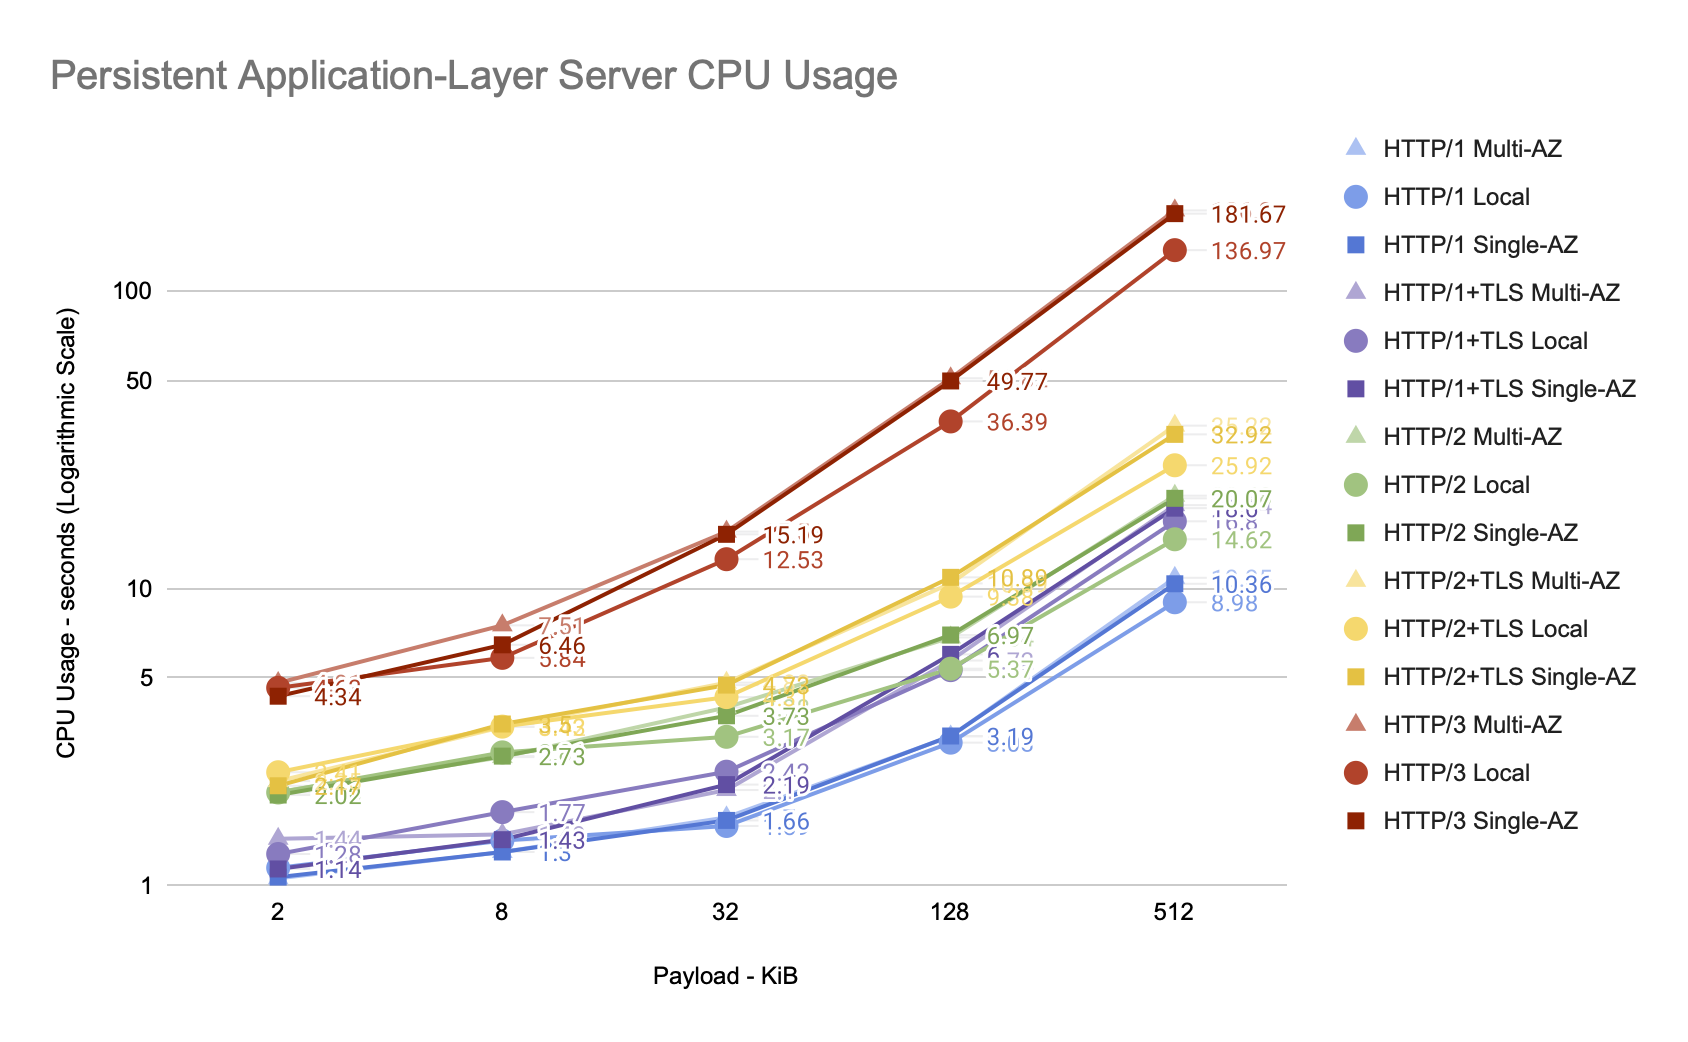
\includegraphics[width=\linewidth]{figures/charts/Persistent Application-Layer Server CPU Usage.png}
    \caption{Persistent Application-Layer Server CPU Usage}
    \label{fig:persistent_server_application_cpu}
\end{figure}

\begin{figure}[h!]
    \centering
    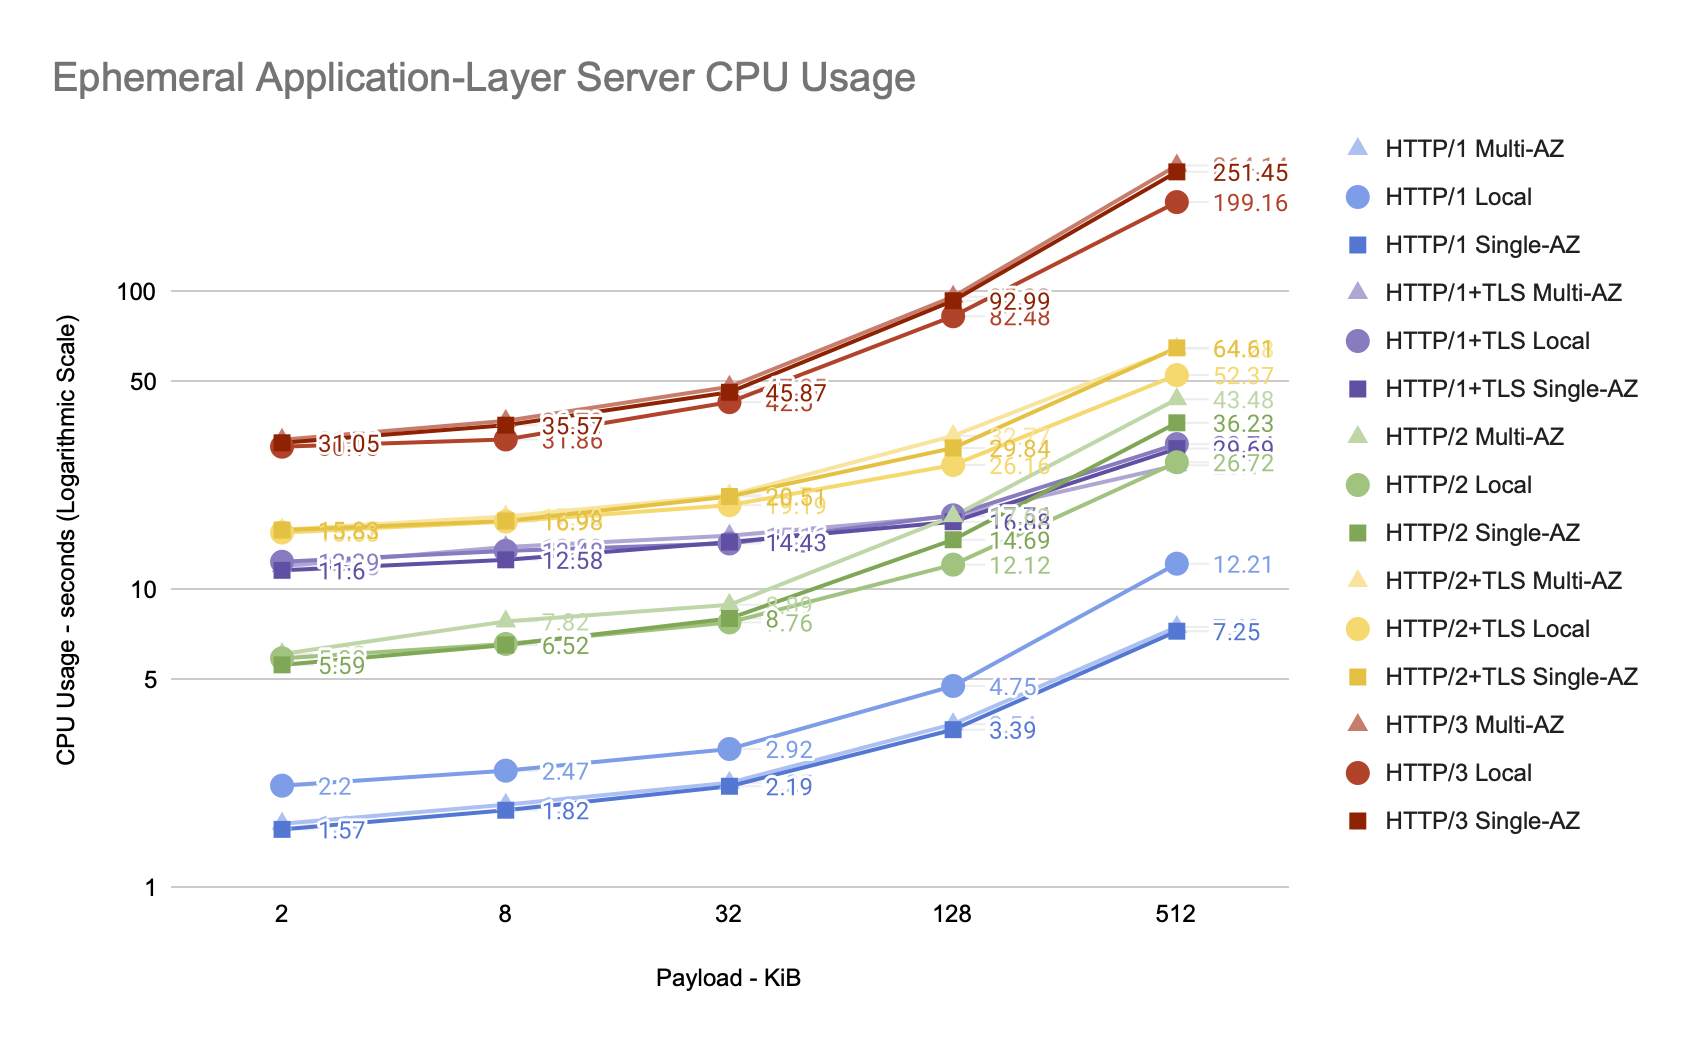
\includegraphics[width=\linewidth]{figures/charts/Ephemeral Application-Layer Server CPU Usage.png}
    \caption{Ephemeral Application-Layer Server CPU Usage}
    \label{fig:ephemeral_server_application_cpu}
\end{figure}

% \begin{figure}[h!]
%     \centering
%     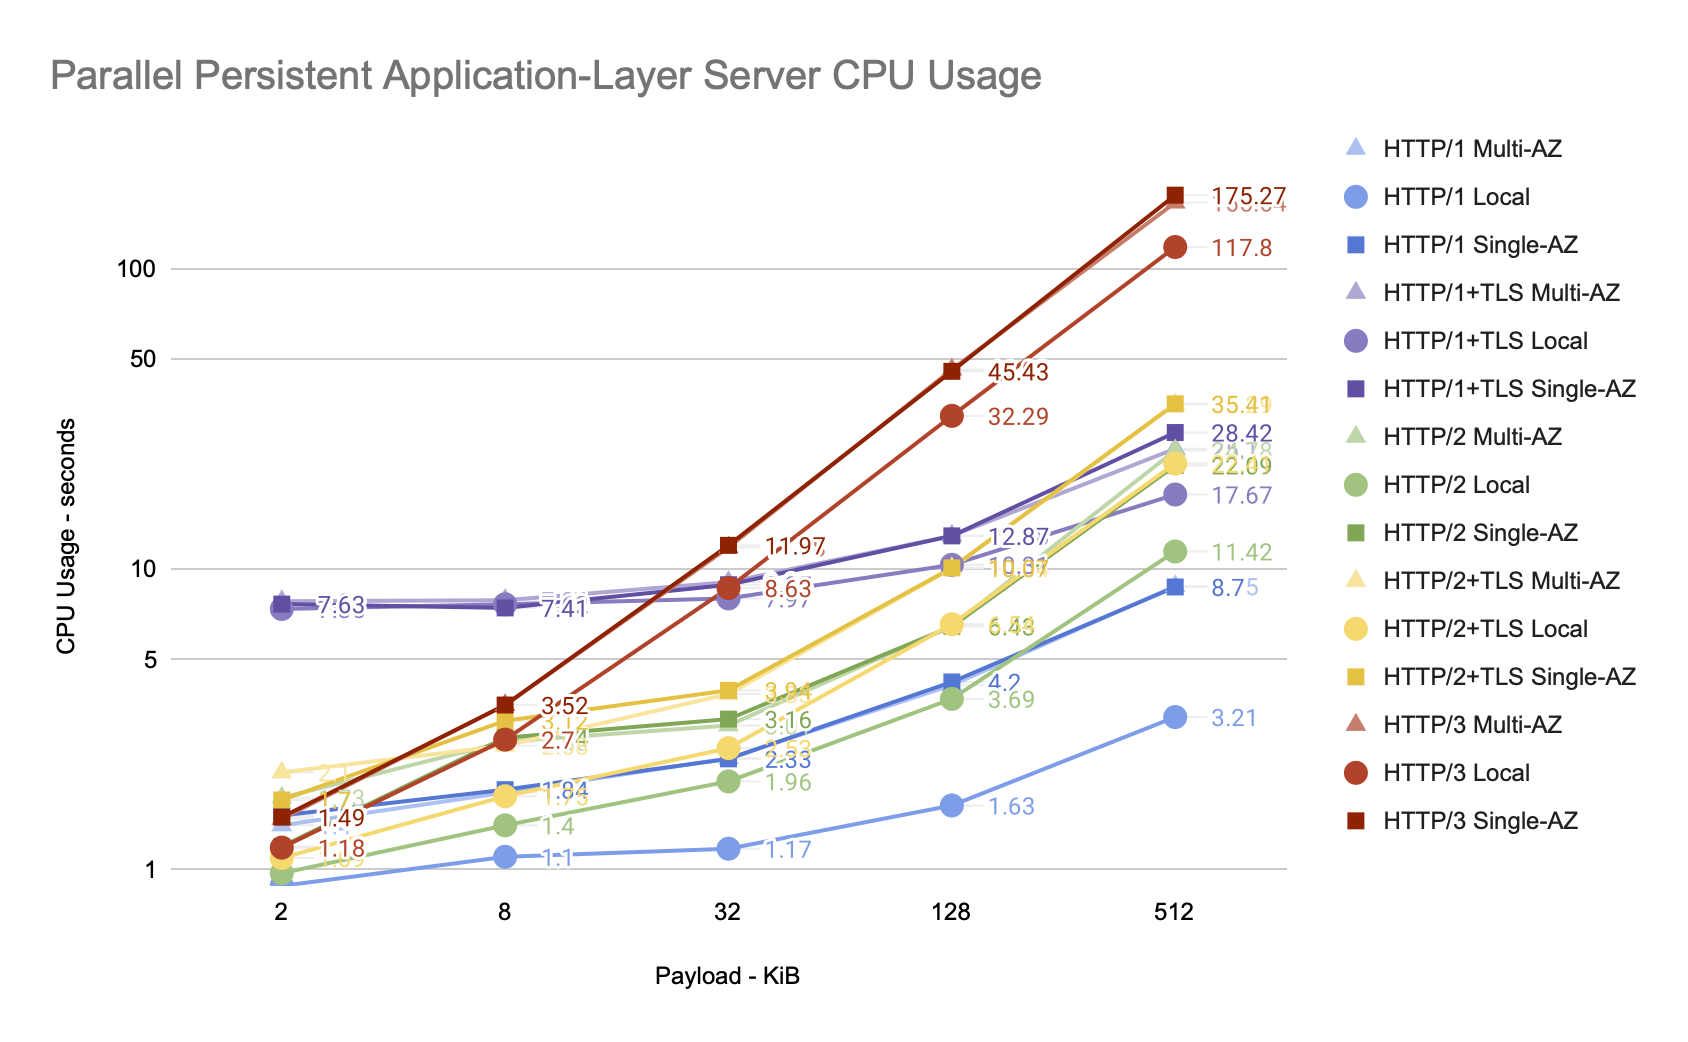
\includegraphics[width=\linewidth]{figures/charts/Parallel Persistent Application-Layer Server CPU Usage.png}
%     \caption{Parallel Persistent Application-Layer Server CPU Usage}
%     \label{fig:parallel_server_application_cpu}
% \end{figure}
